For future work, we plan on using a genetic algorithm (GA) to train the autoencoder's weight matrix and biases. A GA is a black-box optimization algorithm that iteratively improves upon a population of candidate solution vectors until the global optima of the objective function is reached \cite{srinivas1994genetic}. It uses operators such as mutation and crossover, which are inspired by biological evolution. GAs are superior when compared to SGD in training autoencoders in two aspects: 1) Since the loss function is highly nonconvex, SGD will always converge to a local minima, while GA are capable of eventually reaching the global optima. 2) SGD is not trivial to parallelize; as seen by our experimental results, SGD does not achieve linear speedup. On the other hand, GAs are much simplier to parallelize in one of two following ways \cite{cantu1998survey}: a) Each individual in a population can be evaluated in parallel. b) The mutation and crossover operators operate on each element of a solution vector independently and thus are embarrassing parallel. An overview of how genetic algorithms work is given by Algorithm \ref{alg:genetic}. For autoencoders, each individual in the population is some particular weight matrix and its two associated bias vectors. The objective function would be the loss function described earlier and the fitness is how small the error outputted by the loss function is. 

\begin{figure}[h]
\centering
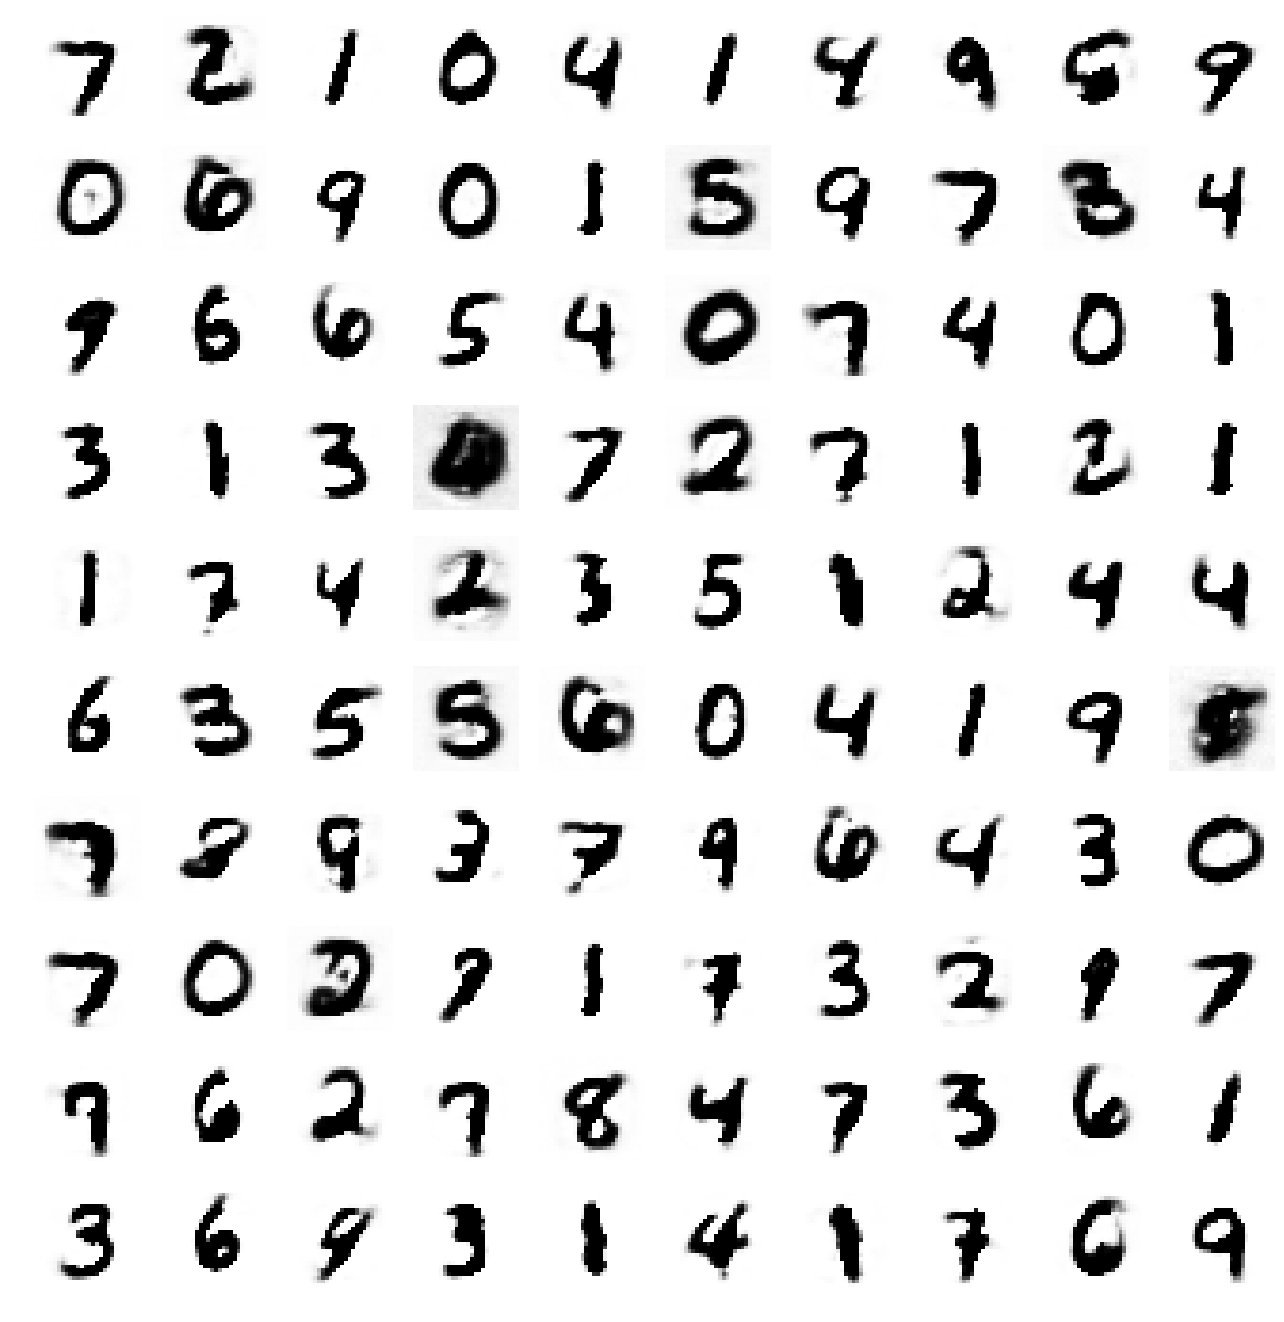
\includegraphics[width=1.0\linewidth]{experiment3_2.png}
\caption{Visualization of the reconstruction capabilities of an denoising autoencoder with 500 hidden units. Odd columns show noisy digit input images, even columns show reconstructed outputs.}
\label{fig:experiment3_2}
\end{figure}

We also plan on evaluating the performance of our autoencoder on additional harder image datasets mentioned in \cite{vincent2010stacked}, such as \textit{bg-rand, bg-img-rot}, which contain images with noise and rotation. 

